\chapter{Implementación.}
\section{Breve introducción a CUDA.}
Como comentábamos al principio, CUDA \textit{(Computer Unified Device Arquitecture)} \cite{cuda} es una tecnología propietaria desarrollada por \textit{NVIDIA} y lanzada en junio de 2007, que nos proporciona de un lenguaje de programación general destinado a ser ejecutado en las tarjetas gráficas de la compañia. Para los propósitos de este trabajo y, habitualmente, a la hora de trabajar con CUDA denominaremos como \textbf{\textit{host}} a la CPU que se comunica con la tarjeta gráfica y como \textbf{dispositivo} a la GPU o tarjeta gráfica utilizada. \\

La intercomunicación entre \textit{host} y dispositivo sigue un modelo maestro-esclavo. El \textit{host} actúa como maestro y es el encargado de indicar al dispoistivo el código que ha de ejecutar y de mandarlo a la cola del dispositivo. Además, el \textit{host} tiene la posibilidad de trabajar de forma asíncrona con la GPU mientras la cola de trabajos del dispositivo no esté llena. \\

Es de vital importancia a la hora de trabajar con la GPU de tener en cuenta que:\\
\begin{itemize}
    \item a) La GPU tiene muchos más núcleos \textit{(cores)} que una CPU, lo que nos permite realizar mucha más operaciones en el mismo instante. Sin embargo, esto viene a expensas de un menor número de operaciones por segundo de cada núcleo, ya que para distrutar de la cantidad masiva de núcleos que tiene una GPU es necesario que ésta opere a una frecuencia más baja.

    \item b) La GPU tiene su propia estructura de memoria, que ha de usar para poder realizar operaciones. Dentro de la jerarquía de memoria encontramos memoria RAM similar a la que utiliza la CPU a través de la placa base, así como varios niveles de caché. Además, hemos de tener en cuenta que a la hora de ejecutar algo en la GPU vamos a tener un gasto extra de tiempo por el traspaso de información de CPU a GPU y viceversa. Minimizar la información que ha de traspasarse en ambos sentidos así como intentar que toda la información necesaria sea transferida a la vez para sacar máximo potencial del PCI Express y exprimir al máximo posible el uso eficiente de la memoria caché, que en CUDA es habitualmente realizado mediante el manejo de la ``memoria compartida'' es fundamental para obtener mejores resultados, especialmente, aquellos en los que el cuello de botella es la transferencia de datos.

    \item c) Como la GPU tiene su propia memoria dedicada de un tamaño limitado hemos de hacer hincapié en no utilizar soluciones que generan demasiada complejidad espacial, ya que limitan la escalabilidad de los algoritmos.
\end{itemize}

\subsection{Estructura de hebras, bloques y mallas.}
El \textbf{\textit{kernel}} es un fragmento de código especial destino a ser ejecutado en el dispotivo en el que se indica lo que ha de hacer una hebra.\\

Las \textbf{hebras} son la unidad mínima en la arquitectura CUDA. Cada hebra es ejecutada por un núcleo CUDA. Cada hebra es consciente en tiempo de ejecución de su identificador dentro del bloque así como del identificador del bloque en el que se encuentra y el tamaño del mismo, permitiéndonos así repartir el trabajo en función de dichos valores. El \textbf{bloque} se corresponde a un conjunto de hebras que ejecuta el mismo \textit{kernel} y que pueden cooperar entre sí y, al conjunto de esos bloques, se le denomina \textbf{``grid'' o malla}. Tanto las hebras dentro de un bloque como los bloques dentro de una malla puede tener estructuras unidimensionales, bidimensionales y tridimensionales. Las dimensiones de estas estructuras será indicada por el \textit{host} a la hora de ejecutar el \textit{kernel}.\\

CUDA exige que un mínimo de 32 hebras, denominado \textit{warp}, ejecuten instrucciones a la vez, aunque se hagan cálculos innecesarios así como que todas las hebras de un bloque sean ejecutadas por el mismo \textit{Streaming MultiProcessor}, de ahora en adelante, SM, que es uno de los procesadores en el dispositivo y dispone de un número específico de núcleos CUDA, sus propios registros y su propia caché entre otros.\\

Al lanzar un \textit{kernel} hemos de utilizar al menos un bloque de $N$ hebras. Además, en los casos unidimensionales el número de hebras por bloque está limitado a un máximo que depende de la tarjeta gráfica en cuestión.

\subsection{La memoria compartida.}
Dentro de la tarjeta gráfica, nos encontramos con distintos niveles de memoria. Una vez los datos necesarios han sido traspasados del \textit{host} al dispositivo a través del bus PCI Express, esos datos son almacenados en una memoria DRAM de propósito general del dispositivo. Cuando un \textit{kernel} solicita datos de esta memoria, de manera similar a como ocurre en una CPU, los datos solicitados y los colidantes en memoria son colocados a través de varios niveles de caché, que tiene tamaño más limitado que la memoria DRAM pero con un acceso de lectura y escritura mucho más rápido.\\

La \textbf{memoria compartida} es una abstracción para una región especial de la caché asociada a un bloque que es explícitamente usada por el programador en el \textit{kernel}, agilizando así considerablemente las transferencias de memoria en el dispositivo. En el cuadro \ref{tab:cudamemory}, podemos ver un resumen de los tipos de memoria existentes, dónde se pueden usar y dónde se encuentran dichos datos en el dispositivo.

\begin{table}[ht]
\begin{tabular}{|c|c|c|c|}
\hline
\textbf{Memoria}    & \textbf{Localización}                                           & \textbf{\begin{tabular}[c]{@{}c@{}}Acceso\\ (E = Escribir)\\ (L = Leer)\end{tabular}} & \textbf{\begin{tabular}[c]{@{}c@{}}Existente\\ hasta fin\\ de\end{tabular}} \\ \hline
\textbf{Registro}   & Caché                                                           & Kernel (E/L)                                                                          & Hebra                                                                       \\ \hline
\textbf{Local}      & \begin{tabular}[c]{@{}c@{}}DRAM\\ (Caché tras uso)\end{tabular} & Kernel (E/L)                                                                          & Hebra                                                                       \\ \hline
\textbf{Compartida} & Caché                                                           & Kernel (E/L)                                                                          & Bloque                                                                      \\ \hline
\textbf{Global}     & \begin{tabular}[c]{@{}c@{}}DRAM\\ (Caché tras uso)\end{tabular} & \begin{tabular}[c]{@{}c@{}}Host (E/L)\\ Kernel (E/L)\end{tabular}                     & \begin{tabular}[c]{@{}c@{}}Aplicación\\ o uso de free\end{tabular}          \\ \hline
\textbf{Constante}  & \begin{tabular}[c]{@{}c@{}}DRAM\\ (Caché tras uso)\end{tabular} & \begin{tabular}[c]{@{}c@{}}Host (E/L)\\ Kernel (L)\end{tabular}                       & \begin{tabular}[c]{@{}c@{}}Aplicación \\ o uso de free\end{tabular}         \\ \hline
\end{tabular}
\caption{Resumen de los tipos de memoria en CUDA.}
\label{tab:cudamemory}
\end{table}

\subsection{Python: Numba y CuPy.}
Para desarrollar el código asociado a este proyecto, hemos optado por utilizar \textbf{Python} en vez de los tradicionales C o C++. El uso de \textit{Python} nos permite un desarrollo de los algoritmos más rápido así como el acceso a abstracciones de más alto nivel mediante el uso de la librerías \textbf{\textit{Numba}} y \textbf{\textit{CuPy}},  así como una mayor facilidad para la distribución del código, si se desea, mediante el uso de \textit{PyPI(Python Package Index)}, el repositorio de paquetes para Python. \\

\textbf{Numba} \cite{numba} es un paquete para Python cuyo objetivo es la aceleración compilado fragmentos de código utilizando el compilador LLVM y dando la oportunidad de paralelizar código tanto para la CPU como para la GPU. En concreto, para las GPUs CUDA, proporciona al usuario un subconjunto de las características de CUDA con un nivel de abstracción mayor. Con eso no sólo conseguimos poder trabajar con CUDA desde Python sino, también evitar, si lo deseamos, manejar los traspasos de memoria entre host y dispositivo o la necesidad de indicar todos los tipos a la hora de inicializar un \textit{kernel} entre otras ventajas.
\begin{code}
\begin{minted}[fontsize=\footnotesize]{python}
from numba import cuda
import numpy as np
# Definimos el kernel
@cuda.jit
def aumentar_en_1(un_array):
  # Cogemos el índice de la hebra
    pos = cuda.grid(1)

    # Si el índice está en el rango del array
    # incrementamos su valor
    if pos < un_array.size:
        un_array[pos] += 1

if __name__ == '__main__':
  # Declaramos un array de 10000 ceros
  ejemplo = np.zeros(10000)
  # Calculamos el número de bloques necesario
  bloques = ejemplo.size // 128 + 1
  # Lanzamos el kernel con bloques de 128 hebras
  aumentar_en_1[bloques, 128](ejemplo)
\end{minted}
\captionof{listing}{Kernel para incrementar en 1 los elementos de un array.\\\\}
\label{code:numbaexample}
\end{code}

\textbf{CuPy} \cite{cupy} es otro paquete de Python que, por un lado y de manera similar a Numba, nos permite generar kernels para CUDA en este caso de manera similar a los de C/C++ así como facilidades para generar kernels en los que se implementa reducciones u operaciones elemento a elemento en un array. Por otro lado, proporciona una API similar a la de NumPy pero las operaciones están implementadas utilizando CUDA. Además, CuPy está implementado de manera que permite utilizar directamente sus estructuras de datos sobre kernels de Numba, lo que nos permite combinar elementos de ambos paquetes según nos interese.

\subsection{Spark.}
\textit{Apache Spark} es un \textit{framework} de código abierto y propósito general para sistemas distribuidos de computación en clúster que proporciona una API utilizable desde los lenguajes de programación en Scala, Java, Python y R. El \textit{framework} fundamenta su arquitectura en el \textit{RDD (Resilient Distributed DataSet)}, que es una estructura de datos de sólo lectura distribuida en un clúster de máquinas, mantenida durante toda la computación y con tolerancia a fallos. Además, proporciona otras herramientas de alto nivel como ML/MLib, una librería con algoritmos de \textit{machine learning}.\\

Utilizando la API de Python, podemos combinar el uso de \textit{Spark} y \textit{Numba CUDA} para afrontar problemas de grandes dimensiones, ya que el \textit{RDD} nos permite trabajar con subconjuntos de esos datos posibilitando incluso llevar las implementaciones realizadas a un clúster con múltiples sistemas con dispositivos GPU \textit{CUDA} cont todas las dependencias necesarias instaladas. \\

La distribución de trabajo en Spark se realizará utilizando la transformación \textit{mapPartitions} del \textit{RDD} de \textit{Spark}, que generá un nuevo RDD a partir de los resultados obtenidos al aplicar la función pasada a \textit{mapPartitions} como parámetro a cada una de las funciones.


\section{Proceso de implementación.}
Para realizar la implementación de cada algoritmo hemos realizado un proceso cíclico divido en 3 fases:

\begin{itemize}
	\item \textbf{Análisis} - En la primera iteración, analizar los trabajos relacionados. En las posteriores, analizar los resultados obtenidos del profiler, determinar los cuellos de botella y buscar posibles alternativas para solucionar el problema.
	\item \textbf{Implementación} - Realizar la implementación en CUDA de los cambios o elementos nuevos obtenidos del proceso de análisis.
	\item \textbf{Profiling} - Utilizar el profiler de NVIDIA, \textit{Nsight}, sobre un ejemplo razonable para evaluar el rendimiento del algoritmo.
\end{itemize}

En este capítulo, explicaremos las soluciones finales a las que hemos llegado y destacaremos algunas de las decisiones tomadas y el razonamiento para haberlas seleccionado. Para facilitar la comprensión y tener en cuenta las dependencias de datos de los algoritmos durante el proceso de desarrollo hemos utilizado diagramas de flujo adaptados que nos permitan tener una visión general de las dependencias existentes entre los procesos y datos de una manera esquemática para cada uno de los modelos. 

\section{Desarrollo del mapa autoorganizado de Kohonen.}
Para implementar los mapas autoorganizados de Kohonen, primero consideramos la versión tradicional \textit{online} y, posteriormente, tras ver las limitaciones de la primera, evaluamos la versión computada en \textit{batchs}. Ambas implemntaciones ha sido realizadas tanto para CPU como para CUDA. El código desarrollado en la versión para CPU ha sido realizado en \textit{Python} usando \textit{NumPy} conforme a lo explicado al presentar el modelo. En este capítulo, nos centramos en la implementación realizada en \textit{CUDA}.

\subsection{Limitaciones del mapa autoorganizado online.}
Mientras que la implementación del mapa autoorganizado \textit{online} fue el punto de partida para la realización de este trabajo tuvimos que descartar esta versión del algoritmo, ya que, el objetivo de este trabjo es resolver problemas con un gran número de muestras utilizando \textit{CUDA} y \textit{Spark}.\\

En esta versión, en cada iteración, se selecciona una única muestra del conjunto de datos y ésta es evaluada para actualizar los pesos de las neuronas, que serán el punto de partida de la siguiente iteración, limitando a una el número de muestras que pueden procesarse a la vez y, por tanto, secuencializando el proceso.\\

La opción más apropiada para paralelizar este algoritmo, sería procesar una única muestra usando tantas hebras como neuronas tenga el mapa de salida. En ese caso, en cada iteración, cada hebra podría calcular su distancia euclídea de la muestra con los pesos de la neurona asociada a la hebra, usaríamos el algoritmo de la reducción (que explicaremos posteriormente) para encontrar la BMU y, cada hebra, realizaría la actualización de los pesos de su neurona, si procediera. Sin embargo, este procedimiento sólo conseguiría ganancias significativas con respecto a su versión para CPU con un mapa de neuronas considerablemente grande, factor que no parece razonable en un algoritmo cuyo principal uso es el \textit{clustering}.\\

Determinadas estas limitaciones y, dado que nuestro objetivo es evaluar un conjunto con un número de muestras elevado, optamos por implementar la versión del mapa autoorganizado que nos permite evaluar múltiples muestras simultáneamente, el mapa autoorganizado \textit{batch}.

Para el desarrollo de esta versión del algoritmo hemos combinado el uso de \textit{CUDA} mediante \textit{Numba} y \textit{Spark}. En primer lugar, vamos a ver un esquema general del uso de \textit{Spark} para afrontar nuestro algoritmo iterativo y, a continuación, explicaremos en detalle la implementación de los \textit{kernels} para \textit{CUDA}.

\subsection{Uso de Spark.}
Utilizar \textit{Spark} para implementar este algoritmo nos permite tanto afrontar problemas de tamaños superiores a la capacidad de memoria de nuestro dispositivo como llevar la implementación realizada a un clúster con múltiples nodos con acceso a un dispositivo \textit{CUDA} que tengan todas las dependencias de \textit{software} instaladas.\\

\begin{figure}[ht]
\centering
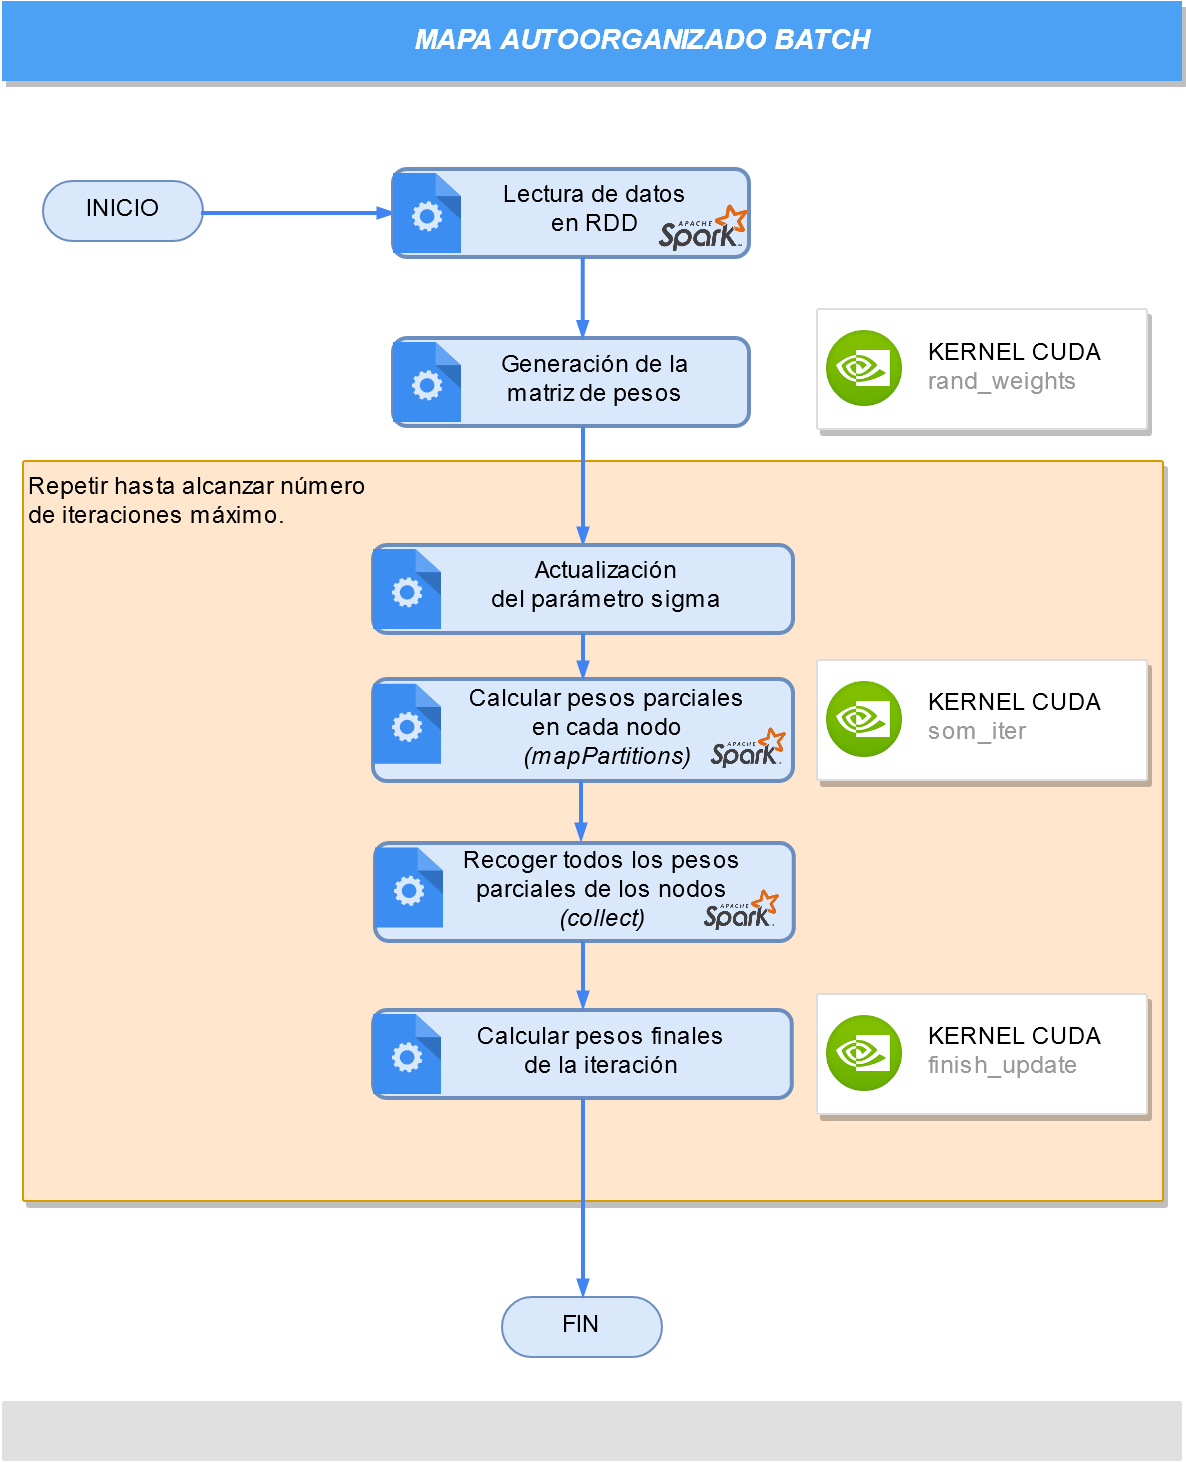
\includegraphics[scale=0.5]{imagenes/flujosparksom.png}
\caption{Diagrama de flujo del mapa autoorganizado desarrollado.}
\label{image:flujosparksom}
\end{figure}

El algoritmo empieza en un único nodo de \textit{Spark} utilizando el primer kernel desarrollado, \textit{rand\_weights}, para inicializar de manera pseudoaleatoria los valores de la estructura de pesos en función de una semilla proporcionada por el usuario. Con esta estructura ya generada, empieza el proceso iterativo en el que:
\begin{itemize}
    \item 1) Calculamos el párámetro de control $\sigma$ para la iteración en función de las ecuaciones correspondientes.
    \item 2) Utilizando la función \textit{mapPartitions}, a cada partición del \textit{RDD} le aplicamos una función que encapsula otro \textit{kernel} desarrollado, \textit{som\_iter}, que se encarga de evaluar la suma parcial de los numeradores y denominadoresde la actualización de pesos para cada neurona en función de las muestras asociadas a la partición del \textit{RDD}.
    \item 3) Para finalizar la iteración, \textit{Spark} reúne mediante \textit{collect} las sumas parciales obtenidas y, usando el último \textit{kernel} implementado, \textit{finish\_update} obtiene los pesos finales de la iteración.
\end{itemize}

Este proceso, que contiene 3 fases, es realizado hasta alcanzar el número máximo de iteraciones. Hemos de destacar que, puesto que todas las particiones han de partir de la mismos pesos de las neuronas en cada iteración. Por ello, al incicio de la iteración, es necesario distribuir la matriz de pesos a cada nodo de \textit{Spark} que realiza los cálculos de una partición y, al final de la iteración, reunir todos los pesos parciales en un único nodo, permitiéndonos obtener los pesos finales de la iteración. \\

Sin embargo, para que \textit{Spark} pueda realizar esa distribución a lo largo del clúster es necesario que, al final de la iteración, se haga la transferencia de memoria de dispositivo a \textit{host} de los pesos parciales y, al inicio de la iteración, se haga la transferencia de \textit{host} a dispositivo de la pesos de las neuronas correspondientes a esa iteración.

\begin{code}
\begin{minted}[fontsize=\footnotesize]{python}
def spark_gpu_batch_som(rdd_data, d, max_iters, rows, cols, smooth_iters=None,
                        sigma_0=10, sigma_f=0.1, tau=400, seed=None, tpb=1024):
    """
    :param rdd_data RDD con el conjunto de muestras a evaluar.
    :param d Tamaño de una muestra, dimensión del problema.
    :param max_iters Número de iteraciones a realizar.
    :param rows Número de filas en el mapa de neuronas.
    :param cols Número de columnas en el mapa de neuronas.
    :param smooth_iters Número de iteraciones en las que el parámetro
           sigma decrece siguiendo una función gaussiana. 
    :param sigma_0 Valor de sigma inicial.
    :param sigma_f Valor de sigma tras alcanzar la iteración smooth_iters.
    :param tau Valor de tau para la función gaussiana.
    :param seed Semilla pseudoaleatoria para la generación inicial de pesos.
    :param tpb Número de hebras por bloque para la inicialización de pesos y
           la actualización final de los pesos.
    """
    
    # 1. Declaramos la estructura de los pesos.
    d_weights = cuda.device_array((rows, cols ,d), np.float32)

    # 1.2 Usamos Numba para generar los pesos de forma pseudoaleatoria.
    rng_states = create_xoroshiro128p_states(rows * cols * d, seed=seed)
    rand_weights[(d_weights.size) // tpb + 1, tpb](rng_states, d_weights)
     
    # 1.3 Traemos los pesos de la memoria de la GPU a la memoria del host.
    weights = d_weights.copy_to_host()

    # 2. Inicio del proceso iterativo
    for t in range(max_iters):
        # 2.a Actualizamos sigma en función de los tau y la iteración.
        if smooth_iters is None or t < max_iters:
            sigma = sigma_0 * math.exp((-t/tau))
        else:
            sigma = sigma_f
            
        sigma_squared = sigma * sigma
        
        # 2.b Cada nodo del clúster de spark trabajará con un subconjunto
        # de las muestras del RDD para encontrar la BMU y realizar la suma
        # parcial de su ecucación de actualización de pesos.
        out = rdd_data.mapPartitions(gpu_work_iter(weights, sigma_squared))
        
        # 2.c En un único nodo usamos la GPU para juntar todas las sumas 
        #     parciales obtenidas y realizar la división
        out = out.collect()
        numParts = len(out) // 2

        partials = np.concatenate(out)
        finish_update[rows * cols // tpb + 1, tpb](weights, partials, numParts)
       
    # 3. Devolvemos los pesos obtenidos
    return weights
\end{minted}
\captionof{listing}{Uso de Spark para entrenar el mapa autoorganizado.}
\label{code:somspark}
\end{code}

\subsection{Representación de la estructura de pesos de las neuronas.}
La estructura que contiene los pesos de las neuronas se corresponde a un array tridimensional. El primer eje indica la fila que ocupa la neurona en el mapa, el segundo eje indica la columna que ocupa la neurona en el mapa y el último eje la característica del problema a la que queremos acceder.\\

Mientras que nosotros podemos hacer uso de esta abstracción para acceder de manera tridimensional gracias a Numba, en realidad, en el dispositivo CUDA se trata de un array unidimensional \textit{row-major}.


\begin{figure}[ht]
\centering
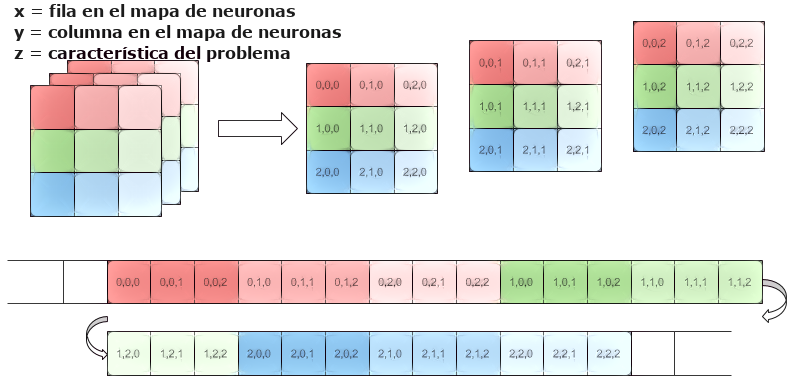
\includegraphics[scale=2.0]{imagenes/row-major.png}
\caption{Representación de un array 3D como un array 1D row-major.}
\label{image:rowmajor}
\end{figure}

\subsection{Kernels implementados.}
\subsubsection{Inicialización pseudoaleatoria de matriz de pesos.}
\begin{code}
\begin{minted}[fontsize=\footnotesize]{python}
@cuda.jit
def rand_weights(rng_states, d_weights):
    """
    Kernel para inicializar aleatoriamente la estructura de pesos con 
    valores en el intervalo [0, 1) tomados de una distribución uniforme
    :param rng_states Estados aleatorios.
    :param d_weigths Vector de filas * columnas * d valores que contendrá 
           los pesos asociados a las neuronas.
    """
    # La hebra coge su identificador unidimensional único.
    idx = cuda.grid(1)

    # La hebra calcula en función del su índice 
    # y cocientes y restos de divisiones entereas
    n_rows, n_cols, d = d_weights.shape

    # Cálculo de la fila (eje X).
    row = idx // (n_cols * d)

    # Cálculo de la columna (eje Y).
    col_d = idx % (n_cols * d)
    col = col_d // d
    # Cálculo de la característica (eje Z).
    i = col_d % d
    
    # Sacamos el aleatorio correspondiente.
    if idx < d_weights.size:
        d_weights[row, col, i] = xoroshiro128p_uniform_float32(rng_states, idx)

\end{minted}
\captionof{listing}{Inicialización aleatoria de la matriz de pesos.\\}
\label{code:numbainitweights}
\end{code}

Este proceso (código fuente \ref{code:numbainitweights}) es realizado por el nodo de Spark que controlaría la ejecución del clúster una única vez al inicio del algoritmo, pero utilizando la GPU. \textit{Numba CUDA} nos proporciona herramientas para la generación de valores flotantes en el rango comprendido entre 0 y 1 basadas en el método de Box-Muller. Hemos utilizado esta herramienta para la generación de nuestra matriz de vectores de pesos inicial. Una vez generados, son trasladados de vuelta a la CPU para ser distribuidos a todos los nodos ejecutores de \textit{Spark}. \\

Al lanzar este kernel, se utilizan tantas hebras como números aleatorios (tabla \ref{tab:randkernel}), distribuidos en bloques de un tamaño indicado por el usuario.
\begin{table}[ht]
\begin{tabular}{@{}lll@{}}
\toprule
\textbf{Kernel}        & \textbf{Nº de Bloques}                                 & \textbf{Nº de hebras por bloque}                                                                       \\ \midrule
\textbf{rand\_weights} & ($filas$ $\cdot$ $columnas$ $\cdot$ $d$) $//$ $tpb$ + 1 & $tpb$ \\ \bottomrule
\end{tabular}

\textit{\\$d=$ dimensión del problema.\\$tpb=$ hebras por bloque (indicados por el usuario).\\ $//=$ cociente de división entera.}
\caption{Parámetro para el lanzamiento del kernel rand\_weights.}
\label{tab:randkernel}
\end{table}



\subsubsection{Cálculo de las distancias euclídeas entre todas las muestras y los pesos.}
El cálculo de la distancia euclídea es una operación masiva uno a uno realizada con todas las muestras de entrada con cada uno de los vectores que representa los pesos de las neuronas del mapa. Para optimizar este operación en \textit{CUDA} hemos realizados dos optimizaciones. Por un lado, puesto que nuestro objetivo final es encontrar la posición de la combinación muestra-neurona con la distancia mínima podemos eliminar el cálculo de la raíz cuadrada de la fórmula de la distancia euclídea pues es una operación costosa y no altera la relación de orden generada. Por otro lado, utilizamos la memoria compartida para asegurarnos de que algunos elementos que son ampliamente utilizados en el bloque permanezca en esa caché de acceso más rápido que la memoria global. En concreto, en este caso, lanzamos una malla bidimenisonal de bloques con tantas filas como número de neuronas y columnas como el número de muestras dividido por el tamaño de un bloque más una. Dada esta distribución, en el mismo bloque estamos calculando la distancia entre la neurona con el asociado a la fila en la malla y el subcojunto de muestras asociada a la columna de la malla. Puesto que los pesos de la neurona son utilizados en todo su bloque, éstos son cargados en la memoria compartida del bloque.


\begin{code}
\begin{minted}[fontsize=\footnotesize]{python}
@cuda.jit
def euclidean_distance(samples, weights, distances, nsamples, d):
    # 1. Tomamos los índices que nos correspoden
    neuron_idx = cuda.blockIdx.x
    samples_idx = cuda.blockIdx.y * cuda.blockDim.x + cuda.threadIdx.x
    
    
    # 2. Ponemos los pesos de la neurona en memoria compartida
    shared_weights = cuda.shared.array(shape=0, dtype=numba.float32)
    for i in range(d // cuda.blockDim.x + 1):
        i_stride = i * cuda.blockDim.x
        my_pos = i_stride + cuda.threadIdx.x
        if my_pos < d:
            shared_weights[my_pos] = weights[neuron_idx * d + my_pos]
            
    cuda.syncthreads()
    
    # 3. Procedemos a realizar el cálculo de la distancia si procede
    if samples_idx < nsamples:
        distance = 0.0
        for i in range(d):
            i_distance = samples[samples_idx * d + i] - shared_weights[i]
            distance += i_distance * i_distance
            
        distances[samples_idx, neuron_idx] = distance
\end{minted}
\captionof{listing}{Cálculo de la distancia euclídea.\\}
\label{code:euclideandistance}
\end{code}

\subsubsection{Encontrar la BMU para cada muestra.}
Todas las distancias del subproblema anterior fueron guardadas en una matriz bidimensional donde la fila representa a la muestra y la columna a la neurona. Por tanto, hemos de encontrar el valor en mínimo en cada fila. \\


\begin{figure}[ht]
\centering
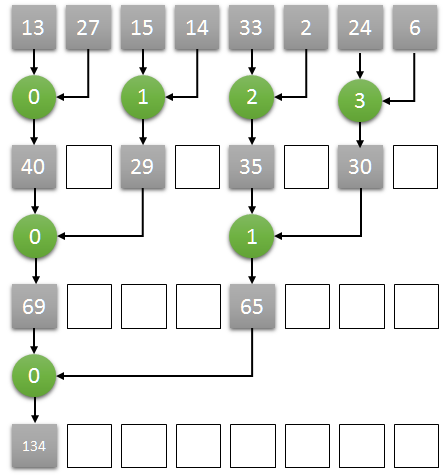
\includegraphics[scale=0.5]{imagenes/parallel_reduce.png}
\caption{Una reducción paralela de una sumatoria en CUDA.}
\label{image:cudareduction}
\end{figure}

Para encontrar el mínimo en un \textit{array} utilizamos un algoritmo frecuentemente utilizando en la GPU: \textbf{la reducción}. Si los elementos de la reducción, caben en un bloque, los mismos son puestos en la memoria compartida del bloque y se simula un recorrido sobre un árbol binario balanceado hacia arriba, tomando los elementos cargadas en memoria compartida como las hojas y alcanzado el resultado final en la raíz. Para que el algoritmo funcione, la operación en cuestión ha de cumplir la propiedad asociativa. Mientras que el uso más habitual de este algoritmo es para realizar la sumatoria nosotros la utilizamos para encontrar el mínimo manteniendo también control del índice que le corresponde. Si todos los datos no caben en un bloque, se lanzan tantos bloques como sean necesarios y este proceso es repetido hasta que queda un único resultado. \\

Puesto que nosotros queremos realizar el proceso para múltiples filas con las mismas dimensiones. Si necesitamos $P$ bloques para resolver la reducción de una fila lanzamos los $N \cdot P$ correspondientes a la vez para obtener la máxima ganancia. Podemos consultar con más detalle cómo realizar una implementación de una reducción de alto rendimiento en \textit{CUDA} en la referencia bibliográfica \cite{reduction}.

\subsubsection{Actualizar la matriz de pesos.}
La fórmula para actualizar cada vector de pesos del mapa depende de dos sumatorias, una en el numerador y otra en el denominador.\\
$$
 W_{i, j} = \frac{\sum_{k=0}^{f} \delta_f(c, [i,j]) \cdot  X(T_k) }{\sum_{k=0}^{f} \delta_f(c, [i,j])}
$$\\

Para utilizar los múltiples nodos ejecutores de \textit{Spark} y sacar el máximo rendimiento, cada nodo realiza la sumatoria de sus muestras guardando el numerador y denominador parciales que les corresponden a sus particiones para, a continuación, ser combinados en el nodo de \textit{Spark} que dirige la ejecución del algoritmo.\\

El cálculo parcial de los numeradores y denominadores parciales se realiza utilizando \textbf{operaciones atómicas}, en concreto, la suma atómica. Las operaciones atómicas son operaciones que sufren de una mayor latencia que su correpondiente operación normal pero evitan condiciones de carrera si múltiples hebras intentan modificar la misma posición de memoria pues realizan la lectura y la actualización del dato en una única operación. La necesidad de utilizar este tipo de operaciones radica en la posibilidad que existe de que la BMU de varias muestras sean la misma neurona y, por tanto, varias hebras intenten modificar la sumatoria de numerador o denominador de la misma neurona al mismo tiempo. Además de esta alternativa, que es por la que hemos optado para realizar el desarrollo de esta parte del algoritmo, podríamos haber generado una estructura auxiliar que para cada neurona contenga $N \cdot d$ entradas para la sumatoria del numerador y otras $N$ para la sumatoria del denominador y posteriormente realizar una reducción con la operación de suma para obtener los resultados deseados. Sin embargo, esta alternativa, como podemos observar, sufriría de una gran complejidad espacial a la hora de afrontar problemas de \textit{Big Data}, limitando la escalabilidad de la solución propuesta a la hora de afrontar problemas de mayor número de muestras o mapas de neuronas más grandes.

Para lanzar nuestro kernel aprovechando la memoria compartida usamos una malla de tantas filas como números de muestras y tantas columnas como 
números de neuronas haya en el mapa divido entre el tamaño del bloque más una. Puesto que los bloques de cada fila de la malla, comprueban si la muestra de la fila está en el rango de actualización de la neuronas que le corresponde a cada bloque mantenemos los datos de la muestra en memoria compartida para asegurarnos de un acceso rápido a los mismos.

\begin{code}
\begin{minted}[fontsize=\footnotesize]{python}
@cuda.jit
def prepare_update(bmu, samples, num, den, 
    nrows, ncols, d, sigma_squared):
    # 1. Tomamos los índices que correspondan
    sample_idx = cuda.blockIdx.x
    neuron_idx = cuda.blockIdx.y * cuda.blockDim.x + cuda.threadIdx.x
   
    # 2. Metemos en memoria compartida la muestra que se lee en todo el bloque
    shared_sample = cuda.shared.array(shape=0, dtype=numba.float32)
    for i in range(d // cuda.blockDim.x + 1):
        i_stride = i * cuda.blockDim.x
        my_pos = i_stride + cuda.threadIdx.x
        if my_pos < d:
            shared_sample[my_pos] = samples[sample_idx * d + my_pos]
    cuda.syncthreads()
    
    # 3. Si procede realizar cálculos los hacemos
    if neuron_idx < nrows * ncols:
        bmu_row = bmu[sample_idx] // ncols
        bmu_col = bmu[sample_idx] % ncols
        neuron_row = neuron_idx // ncols
        neuron_col = neuron_idx % ncols
        
        dist = (neuron_row - bmu_row) * (neuron_row - bmu_row) + \
               (neuron_col - bmu_col) * (neuron_col - bmu_col)
        
        if dist <= sigma_squared:
            hck = math.exp(-dist/(2 * sigma_squared))
            # Guardamos sumatoria del denominador
            cuda.atomic.add(den, neuron_row * ncols + neuron_col, hck)
            # Guardamos sumatoria del numerador
            for i in range(d):
                cuda.atomic.add(num, neuron_row*ncols*d + neuron_col*d+i
                                hck * shared_sample[i])
\end{minted}
\captionof{listing}{Cálculo de numeradores y denominadores parciales.\\}
\label{code:partials}
\end{code}

Una vez todos los resultados han sido recopilados, lanzamos un último kernel que juntará los resultados parciales obtenidos y realizará la división, actualizando los pesos si la neurona en cuestión ha sido BMU de alguna muestra o dejando los pesos de la iteración anterior en caso contrario. En este caso lanzamos una malla unidimensional de tantos bloques como número de neuronas haya entre el tamaño de un bloque más uno. Cada hebra se encarga de realizar las sumas parciales de su neurona asociada y realizar la actualización de su vector de pesos en la matriz si procede.

\begin{code}
\begin{minted}[fontsize=\footnotesize]{python}
@cuda.jit
def finish_update(weights, partials, numParts, nrows, ncols, d):
     idx = cuda.grid(1)
    if idx < nrows * ncols:
        row = idx // ncols
        col = idx % ncols
        
        
        # a) Sumamos todos los parciales en el primer array
        numsize = nrows * ncols * d
        densize = nrows * ncols
        fullsize = numsize + densize
        for i in range(numParts - 1):
            # Suma de numeradores
            for k in range(d):
                pos = fullsize * i + row * ncols * d + col * d + k
                partials[row * ncols * d + col * d + k] += partials[pos]
            # Suma de denominadores
            pos = fullsize * i + numsize + row * ncols + col
            partials[numsize + row * ncols + col] += partials[pos]
            
    cuda.syncthreads()
    
    if idx < nrows * ncols:
        # b) Si no es 0 el denominador realizamos el cambio
        if partials[numsize + row * ncols + col] != 0:
            for k in range(d):
                mypos = row * ncols * d + col * d + k
                denpos = numsize + row * ncols + col
                weights[mypos] =  partials[mypos] / partials[denpos]
\end{minted}
\captionof{listing}{Actualización final de la matriz de pesos.\\}
\label{code:ending}
\end{code}

\subsubsection{Actualizar los parámetros de control.}
Los parámetros de control $\eta$ y $\sigma$ son sólo dos parámetros a modificar por iteración y cuyo cálculo se corresponde a una única operación, por lo que nos es susceptible a ser paralelizado en la GPU y será realizado en el nodo de Spark que dirige la ejecución del clúster si todavía no se ha alcanzado el máximo de iteraciones.
Si se ha alcanzado el máximo de iteraciones el algoritmo termina y la matriz de vectores de pesos de las neuronas de esa última iteración es la solución obtenida.

\begin{figure}[ht]
\centering
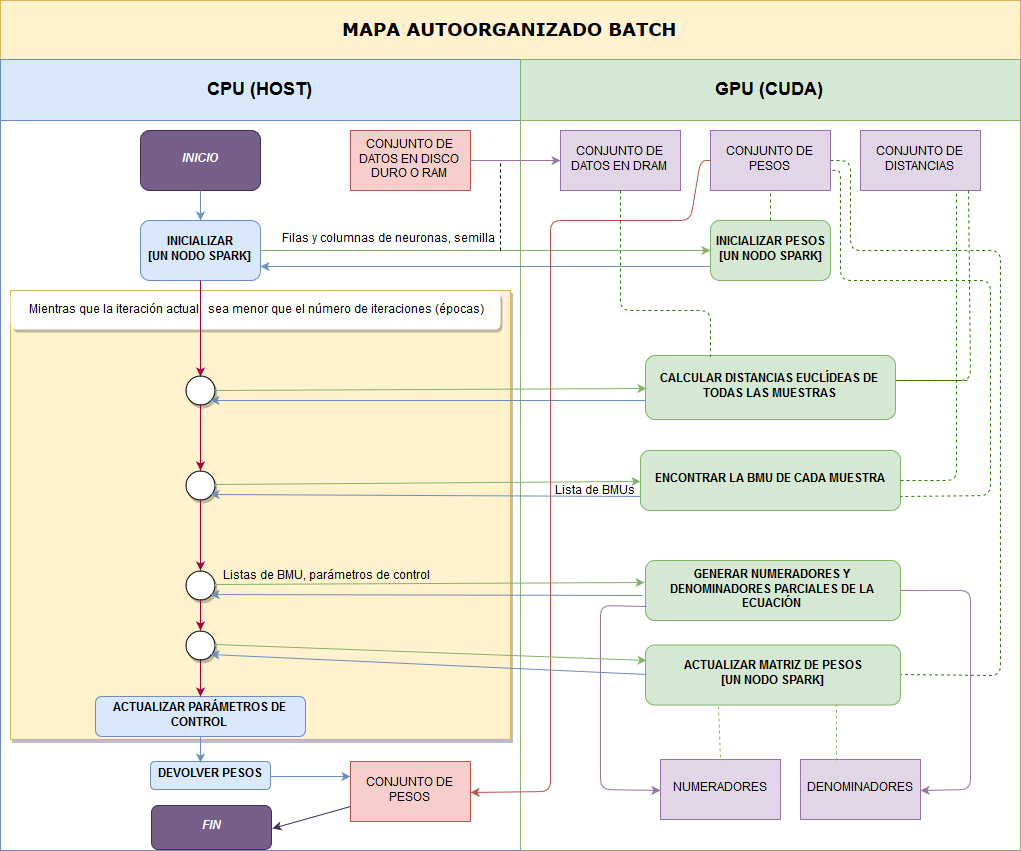
\includegraphics[scale=0.35]{imagenes/flujosombatch.png}
\caption{Diagrama de flujo para el mapa autoorganizado batch.}
\label{img:sombatch}
\end{figure}

\newpage
\section{Desarrollo de un modelo de árbol de decisión.}
La implementación del modelo de árbol de decisión se basa en CUDT \cite{cudt}, que a su vez se fundamenta en SPRINT \cite{sprint} y la operación de \textit{scan}.

\subsection{Lista de atributos.}
Una lista de atributos, es una estructura auxiliar, procedente de SPRINT \cite{sprint}, utilizada para representar las clases y los atributos asociados a una muestra. Una lista de atributos tiene una estructura similar a la siguiente tabla:

\begin{table}[ht]
\centering
\begin{tabular}{@{}lll@{}}
\toprule
Valor & Clase & ID Muestra \\ \midrule
2,5   & 0     & 0          \\
4,7   & 0     & 1          \\
0,1   & 1     & 2          \\
1,0   & 1     & 3          \\ \bottomrule
\end{tabular}
\caption{Una lista de atributos sin ordenar.}
\label{tab:ejlistaatributos}
\end{table}

Las columnas de la tabla \ref{tab:ejlistaatributos} son:
\begin{itemize}
	\item \textbf{Valor}, que se corresponde al valor que toma el atributo al que correponde la tabla en la muestra representada en la fila.
	\item \textbf{Clase}, que se correponde a la etiqueta de salida asoaciada a la muestra de la fila.
	\item \textbf{ID Muestra}, que se correponde al identificador de la muestra. Al principio, se correponde al número de fila empezando por 0.
\end{itemize}

Una vez esta estructura es generada para cada atributo del problema en cuestión, es ordenada por orden creciente según la columna ``Valor''.

\subsection{Esquema general del algoritmo implementado.}
\begin{figure}[ht]
\centering
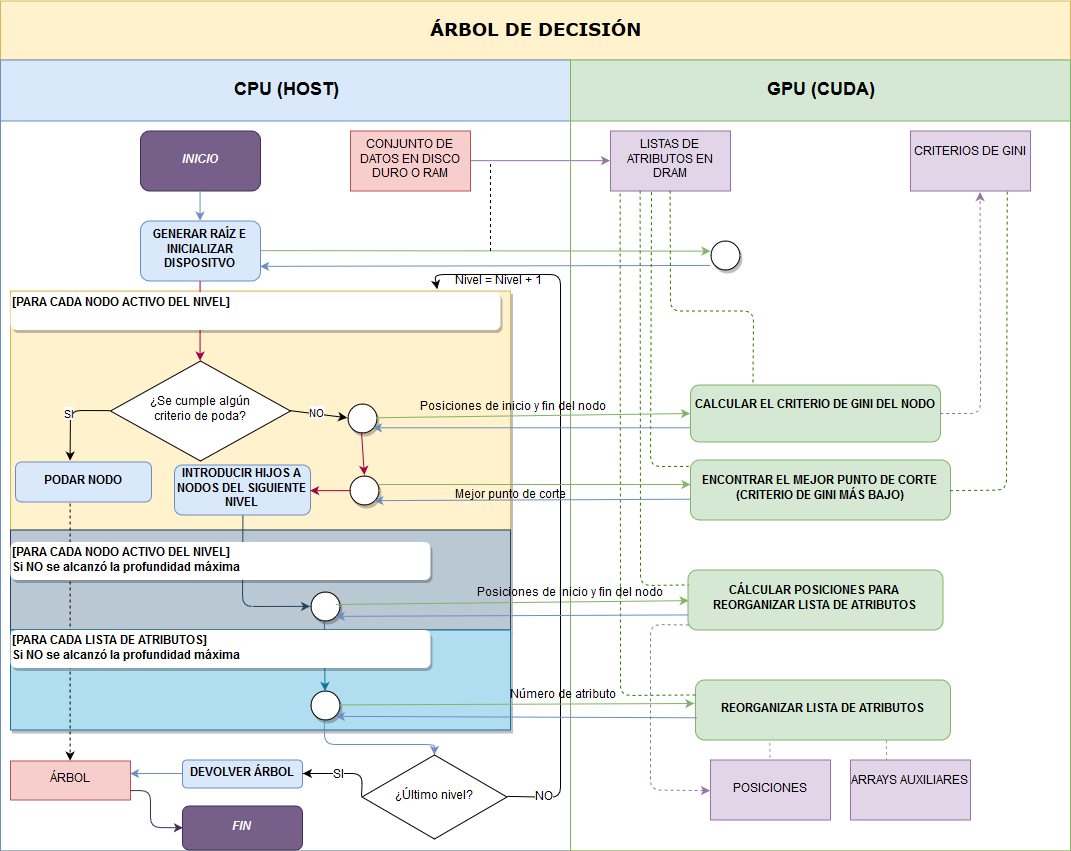
\includegraphics[scale=0.35]{imagenes/esquemadtree.png}
\caption{Diagrama de flujo de la implementación del árbol de decisión.}
\label{img:dtree}
\end{figure}
Al inicio del algoritmo, tras generar las listas de atributos, se genera un nodo raíz que comprende todas las muestras del conjunto. En ese nodo, hemos de encontrar para qué atributo y qué valor realizamos la partición óptima de los datos. Para ello, se consideran todas las listas de atributos y se toma como posible punto de corte el punto medio entre un valor y el siguiente si no se trata del mismo valor. Asociada a cada una de las particiones, se calcula el criterio de Gini. Una vez realizados todos los cálculos, tomamos como punto de corte aquella que menor criterio de Gini nos de. Utilizando ese punto de corte, generamos dos nuevos nodos para la siguiente iteración, uno que contiene todos los puntos menores o iguales que dicho punto de corte y otro con los mayores. Además, dicho punto es el que utilizamos para generar nuestro nodo de decisión en el árbol entrenado.  Este proceso se repite hasta que no quedan nodos por evaluar. Un nodo no ha de ser evaluado si:\\

\begin{itemize}
	\item a) Todos los elementos del nodo pertenecen a la misma clase. En ese caso, en vez de un nodo de decisión, generamos un nodo terminal con la clase correspondiente.
	\item b) Se ha especificado un criterio de profundidad máxima y dicha profundidad ha sido alcanzada. En ese caso, generamos un nodo terminal con la clase más representativa del nodo.
	\item c) Se ha especificado un límite para el número de elementos mínimo que puede contener y ha sido alcanzado. En ese caso, generamos un nodo terminal de manera similar al caso anterior.
\end{itemize}



\subsection{La operación de scan.}
Una de las claves del uso de la lista de atributos, es que, para los problemas de \textbf{clasificación binaria}, que son los únicos que nuestro modelo es capaz de resolver, si codificamos una clase como $0$ (a partir de ahora llamada \textit{clase negativa}) y otra como $1$ (\textit{clase positiva}) si realizamos una suma acumulada sobre el subconjunto de filas de un nodo de la columna ``Clase'' podríamos tener control de cuántos elementos hay en cada clase tanto para todas las particiones. Para realizar la suma acumulada existe un algoritmo ampliamente utilizada en el mundo de la GPU denominado \textit{scan}.

El \textit{scan} \cite{scan}, suma acumulada o suma prefija, es una operación que utiliza un operador binario, $\oplus$, que cumpla la propiedad asociativa y utilizada sobre un \textit{array} de $n$ elementos. Existen dos formas de realizar el \textit{scan}: inclusivo y exclusivo. El scan inclusivo empieza con el primer elemento del array y va a realizando una suma acumulada. El \textit{scan} exclusivo empieza con el elemento neutro de la operación y realiza una suma acumulada de todos los elementos hasta el penúltimo. En la implementación realizada hemos utilizado una operación de \textit{scan} exclusivo que además devuelve el total de la suma del array cubriendo ambos casos. Para los propósitos de este documento, cada vez que hablemos de \textit{scan} nos estaremos refiriendo al \textit{scan exclusivo}. Por tanto la operación de \textit{scan} sobre un array nos devuelve lo siguiente:

$$scan([a_0, a_1, a_2, ..., a_{n-1}]) = [I, a_0, (a_0 \oplus a_1), (a_0 \oplus a_1 \oplus a_2), ..., (a_0 \oplus a_1 \oplus a_2 \oplus ... \oplus a_{n-1})]$$

La implementación en \textit{CUDA} de la operación se realiza, utilizando una técnica frecuente para estos dispositivos, simular el uso de un árbol binario balanceado utilizando la memoria compartida del bloque. Imaginamos que todos los elementos de un bloque son los nodos terminales de un árbol y los metemos en la memoria compartida del bloque y realizamos dos fases sobre ello. En la primera fase, \textit{up-sweep} (figura \ref{image:upsweep}), se realiza el recorrido de los nodos terminales a la raíz realizando las sumas en sus nodos padre y manteniendo las sumas paciales. En la segunda fase \textit{down-sweep} (figura \ref{image:downsweep}), se utilizan los resultados parciales obtenidos para completar los resultados en la suma acumulada. Para arrays cuya dimensión no cabe en un bloque dicho array es subdividido en múltiples subconjuntos contiguos del mismo tamaño que sí caben en un bloque (si sobran elementos en el último bloque son inicalizados con el elemento neutro de la operación) y se genera el scan sobre todos los subconjuntos así como se almacena la sumatoria (puesto en que nuestra caso la operación es la suma) de todos los elementos del bloque. Una vez finalizado, dichas sumatorias se aplican a los bloques que le preceden en posición, obtiendo el resultado final deseado.


\begin{figure}[ht]
\centering
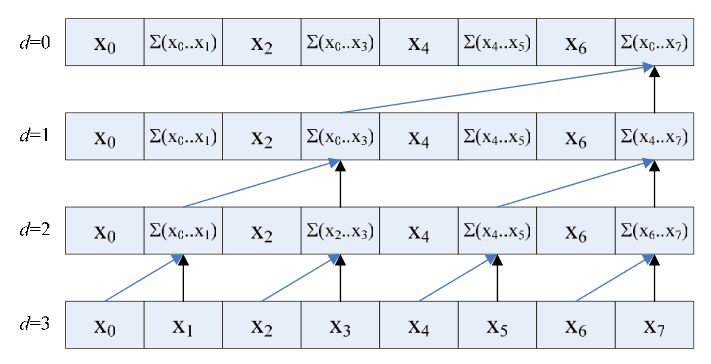
\includegraphics[scale=0.6]{imagenes/upsweep.png}
\caption{Fase up-sweep del scan.}
\label{image:upsweep}
\end{figure}

\begin{figure}[ht]
\centering
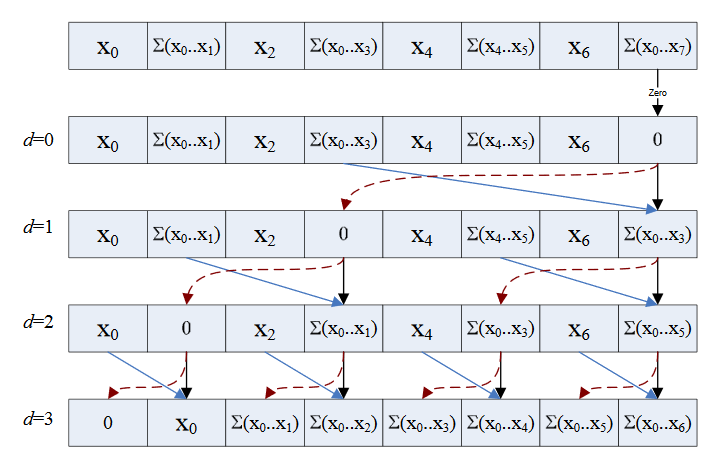
\includegraphics[scale=0.6]{imagenes/downsweep.png}
\caption{Fase down-sweep del scan.}
\label{image:downsweep}
\end{figure}


\subsection{Cálculo del criterio de Gini.}
Dado que sólo vamos a calcular el criterio de Gini para problemas de clasificación binaria hemos simplificado el mismo para ahorrarnos algunas operaciones a la hora de realizar el cálculo:

$$CRITERIO(A,v) = \frac{|i: A_i \leq v|}{N} \cdot GINI(|i: A_i \leq v|) + \frac{|i: A_i > v|}{N} \cdot GINI(|i: A_i > v|)$$

$$GINI(D) = 1 - \frac{T_D^2}{N_D^2} - \frac{F_D^2}{N_D^2}$$

Siendo $N_D$ el total de las muestras en el nodo $D$, $T_D$ el total de muestras pertenecientes a la clase positiva y $F_D$ el total de muestras pertenencientes a la clase negativa. Tenemos que:

$$F_D = N_D - T_D$$
Sustituyendo obtenemos que:

$$GINI(D) = \frac{N_D^2-T_D^2- (N_D - T_D)^2}{N_D^2} = \frac{N_D^2 - T_D^2 - (N_D^2+T_D^2 - 2 N_D T_D)}{N_D^2}$$
$$GINI(D) = \frac{-2T_D^2 + 2N_DT_D}{N_D^2} = 2 \frac{T_D(N_D-T_d)}{N_D^2}$$

$$CRITERIO = \frac{N_\leq}{N}\frac{2T_\leq(N_\leq - T_\leq)}{N_\leq^2} + \frac{N_>}{N}\frac{2T_>(N_> - T_>)}{N_>^2}$$
$$CRITERIO = \frac{2}{N}\Big(\frac{T_\leq(N_\leq - T_\leq)}{N_{\leq}} + \frac{T_>(N_> - T_>)}{N_>}\Big)$$

Puesto que además, no es de nuestro interés el valor específico sino obtener el valor óptimo, podemos ahorrarnos la multiplicación por $\frac{2}{N}$. Así pues, calculamos el criterio de la siguiente manera:

$$CRITERIO' = \Big(\frac{T_\leq(N_\leq - T_\leq)}{N_{\leq}} + \frac{T_>(N_> - T_>)}{N_>}\Big)$$

El valor de $CRITERIO'$ oscilará entre 0 y $\frac{N}{2}$ y buscaremos siempre obtener el mínimo valor para este criterio. Dicha búsqueda se realizará de manera similar a la realizada para el modelo anterior con una reducción para encontrar el índice mínimo en cada nodo.

\subsection{Reorganización de la listas de atributos.}
Para finalizar la evaluación de los nodos de un nivel podemos volver a aprovechar la operación de \textit{scan} para reorganizar el orden de los elementos de la lista de atributos sin necesidad de ejecutar ningún algoritmo de ordenación. Una vez se ha seleccionado la combinación de mejor lista de atributos para un nodo y su punto de corte, puesto que esta lista ya estaba ordenada, todos los elementos hasta el punto de corte pertenecen al nodo hijo izquierdo y los posteriores al nodo hijo derecho. Además, puesto que tenemos en la lista de atributos el cammpo ``ID Muestra'', podemos generar fácilmente un array de booleanos donde cada elemento indica si la muestra con el ID asociado a su posición pertenece al hijo izquierdo o al hijo derecho. Una vez hecho esto, podemos recorrer cada nodo activo de la lista de atributos y utilizar este array auxiliar y la operación de scan para determinar la nueva posición que va a ocupar el elemento dentro del nodo. Esto se realiza, aplicando un scan sobre las posiciones de este array que le corresponden a cada muestra del nodo que va a ir a la subdivisión izquierda. De esta manera, si la muestra pertenece a la subdivisión izquierda su nueva posición será la suma acumulada de elementos de la subdivisión izquierda menos uno (porque empezamos a indexar el array en 0) y en caso de pertenecer a la subdivisión de la derecha será la posición más la diferencia del total de elementos de la subdivisión izquierda (suma acumulada total) con la suma acumulada de elementos de la subdivisión izquierda menos uno.

\subsection{Limitaciones y uso de Spark.}
Como comprobaremos posteriormente, este modelo, al requerir de la evaluación independiente de múltiples nodos y no presentar técnicas de poda avanzadas no escala bien con la generación de árboles profundos o completos. Es por eso que, para afrontar problemas de mayores dimensiones, en vez de generar un único árbol, vamos a generar tantas particiones del \textit{RDD} de \textit{Spark} como árboles deseemos y montar un modelo de \textit{random forest}, en el que en cada partición tenemos un conjunto aleatorio de muestras tomadas sin reemplazo y consideramos todos los atributos para todos los árboles. La clasificación proporcionada por el modelo viene dada por el clase mayoritariamente votada por el conjunto de árboles.

